\documentclass{standalone}
\usepackage{tikz}

\begin{document}

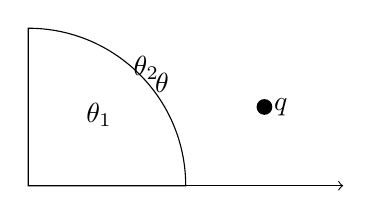
\begin{tikzpicture}[scale=2]
    % Draw the arc for the sector
    \draw (0,0) -- (1,0) arc (0:90:1) -- cycle;
    
    % Label the angles
    \node at (0.45,0.45) {$\theta_{1}$};
    \node at (0.75,0.75) {$\theta_{2}$};
    \node at (0.85,0.65) {$\theta$};
    
    % Draw the arrow
    \draw[->] (1,0) -- (2,0);
    
    % Place the dot and label
    \fill (1.5,0.5) circle (0.05) node[right] {$q$};
\end{tikzpicture}

\end{document}